\documentclass[12pt]{article}
\usepackage{amsmath, amssymb, amsthm, enumerate, graphicx}
\usepackage[usenames,dvipsnames]{color}
\usepackage{bm}
\usepackage[colorlinks=true,urlcolor=blue]{hyperref}
\usepackage{geometry}
\geometry{margin=1in}
\usepackage{float}
\usepackage{graphics}
\setlength{\marginparwidth}{2.15cm}
\usepackage{booktabs}
\usepackage{enumitem}
\usepackage{epsfig}
\usepackage{setspace}
\usepackage{parskip}
\usepackage[normalem]{ulem}
\usepackage{tikz}
\usetikzlibrary{positioning, arrows, automata}
\usepackage{pgfplots}
\pgfplotsset{compat=newest}
\usepackage[font=scriptsize]{subcaption}
\usepackage{float}
\usepackage[]{algorithm2e}
\usepackage{environ}
\usepackage{bbm}
\usepackage{graphicx}
\usepackage{titling}
\usepackage{url}
\usepackage{xcolor}
\usepackage{lipsum}
\usepackage{lastpage}
\usepackage[colorlinks=true,urlcolor=blue]{hyperref}
\usepackage{multicol}
\usepackage{tabularx}
\usepackage{comment}
\usepackage[utf8]{inputenc}
\usepackage{amssymb}
\usepackage{setspace}
\usepackage{marvosym}
\usepackage{wrapfig}
\usepackage{datetime}
\usepackage[many]{tcolorbox}
\usepackage{array}
\usepackage{multirow}
\usepackage{wasysym}
\usepackage{cancel}
\usepackage{cprotect}
\usepackage{listings}
\usepackage{color}

\def\beqa#1\eeqa{\begin{eqnarray}#1\end{eqnarray}}
\newcommand{\R}{{\mathbb{R}}}
\newcommand{\E}{{\mathbb{E}}}
\newcommand{\N}{{\cal{N}}}
\newcommand{\C}{{\cal{C}}}
\newcommand{\D}{{\cal{D}}}
\newcommand{\I}{{\cal{I}}}
\renewcommand{\S}{{\cal{S}}}
\newcommand{\bx}{{\bf{x}}}
\newcommand{\by}{{\bf{y}}}
\newcommand{\bz}{{\bf{z}}}
\newcommand{\bX}{{\bf{X}}}
\newcommand{\br}{{\bf{r}}}
\newcommand{\bt}{{\bf{t}}}
\newcommand{\bo}{{\bf{o}}}
\newcommand{\bp}{{\bf{p}}}
\newcommand{\bl}{{\bf{l}}}
\newcommand{\bw}{{\bf{w}}}
\newcommand{\bv}{{\bf{v}}}
\newcommand{\bq}{{\bf{q}}}
\newcommand{\bh}{{\bf{h}}}
\newcommand{\bS}{{\bf{S}}}
\newcommand{\bM}{{\bf{M}}}
\newcommand{\bR}{{\bf{R}}}
\newcommand{\bphi}{{\boldsymbol{\phi}}}
\newcommand{\bPhi}{{\boldsymbol{\Phi}}}
\newcommand{\bepsilon}{{\bf{\epsilon}}}
\renewcommand{\d}{{\textrm{d}}}
\newcommand{\Figref}[1]{Fig.~\ref{#1}}
\newcommand{\Eqref}[1]{Eq.~\ref{#1}} % The '~' stops breaking and gives correct spacing
\newcommand{\Eqrefs}[2]{Eqs.~\ref{#1},~\ref{#2}}

\newcommand{\norm}[1]{\left\lVert #1 \right\rVert}

\newcommand{\ba}{{\bf{a}}}
\newcommand{\bb}{{\bf{b}}}
\newcommand{\Z}{{\cal{Z}}}
\newcommand{\bmu}{{\boldsymbol{\mu}}}
\newcommand{\bSigma}{{\boldsymbol{\Sigma}}}
\newcommand{\bW}{{\bf{W}}}

\newcommand{\blackcircle}{\tikz\draw[black,fill=black] (0,0) circle (1ex);}
\renewcommand{\circle}{\tikz\draw[black] (0,0) circle (1ex);}

\newtcolorbox[]{solution}[1][]{%
    breakable,
    enhanced,
    colback=white,
    title=Solution,
    fontupper=\color{red},
    #1
}


% SOLUTION environment
\NewEnviron{soln}[1]{
\begin{solution}[#1]
\leavevmode\ignorespaces \BODY 
\end{solution}
}{}

% QUESTION AUTHORS environment
\NewEnviron{qauthor}{
\leavevmode\color{blue}\ignorespaces \textbf{Author} \BODY}{}

% SOLUTION environment
\NewEnviron{qlearningobjective}{
\leavevmode\color{blue}\ignorespaces \textbf{Learning Objective } \BODY }{}

% TO ONLY SHOW HOMEWORK QUESTIONS, include following (else comment out):
\RenewEnviron{soln}[1]{\begin{solution}[#1] \end{solution}}
\RenewEnviron{soln}[1]{\begin{solution}[#1] \BODY \end{solution}}  % Use this for the handout tex
\RenewEnviron{qauthor}{}
\RenewEnviron{qlearningobjective}{}

\renewcommand{\thesection}{Problem \arabic{section}}

%\newcommand{\norm}[1]{\lVert #1 \rVert}
%\newcommand{\st}{\mathrm{s.t.}}

\makeatletter
\newcommand{\removelatexerror}{\let\@latex@error\@gobble}
\makeatother

\newcommand{\argmax}{\mathop{\mathrm{argmax}}}
\newcommand{\argmin}{\mathop{\mathrm{argmin}}}

%%%%%%%%%%%%%%%%%%%%%%%%%%%%%%%%%%%%%%%%%%%
% Custom Math                             %
%%%%%%%%%%%%%%%%%%%%%%%%%%%%%%%%%%%%%%%%%%%


%%%%%%%%%%%%%%%%%%%%%%%%%%%%%%%%%%%%%%%%%%%
% Custom box for highlights               %
%%%%%%%%%%%%%%%%%%%%%%%%%%%%%%%%%%%%%%%%%%%

% Define box and box title style
\tikzstyle{mybox} = [fill=blue!10, very thick,
    rectangle, rounded corners, inner sep=1em, inner ysep=1em]

% \newcommand{\notebox}[1]{
% \begin{tikzpicture}
% \node [mybox] (box){%
%     \begin{minipage}{\textwidth}
%     #1
%     \end{minipage}
% };
% \end{tikzpicture}%
% }

\NewEnviron{notebox}{

\begin{tikzpicture}
\node [mybox] (box){
    \begin{minipage}{\textwidth}
        \BODY
    \end{minipage}
};
\end{tikzpicture}
}


\begin{document}
% Enter your solutions below. For example, to answer "Yes." for problem 1, you should update below as \def \One{Yes}.

% Problem 1
\def \One{
% Please enter your solution here.
}

% Problem 2.1
\def \TwoA {
% Please enter your solution here.
}

% Problem 2.2
\def \TwoB {
% Please enter your solution here.
}

% Problem 3.1.1
\def \ThreeAA {
% Please enter your solution here.
}

% Problem 3.1.2
\def \ThreeAB {
% Please enter your solution here.
}

% Problem 3.2.1
\def \ThreeBA {
% Please enter your solution here.
}

% Problem 3.2.2
\def \ThreeBB {
% Please enter your solution here.
}

% Problem 3.3.1
\def \ThreeCA {
% Please enter your solution here.
}

% Problem 3.3.2
\def \ThreeCB {
% Please enter your solution here.
}

% Problem 3.4
\def \ThreeD {
% Please enter your solution here.
}

% Problem 4.1
\def \FourA {
% Please enter your solution here.
}

% Problem 4.2.1
\def \FourBA {
% Please enter your solution here.
}

% Problem 4.2.2
\def \FourBB {
% Please enter your solution here.
}

% Problem 4.2.3
\def \FourBC {
% Please enter your solution here.
}

% Problem 4.3.1
\def \FourCA {
% Please enter your solution here.
}

% Problem 4.3.2
\def \FourCB {
% Please enter your solution here.
}

% Problem 5.2.1
\def \FiveBA {
% Please enter your solution here.
}

% Problem 5.2.2
\def \FiveBB {
% Please enter your solution here.
}

% Problem 5.2.3
\def \FiveBC {
% Please enter your solution here.
}

% Problem 5.2.4
\def \FiveBD {
% Please enter your solution here.
}

% Problem 6.2.1.1
\def \SixBAA {
% Please enter your solution here.
}

% Problem 6.2.1.2
\def \SixBAB {
% Please enter your solution here.
}

% Problem 6.2.1.3
\def \SixBAC {
% Please enter your solution here.
}

% Problem 6.2.1.4
\def \SixBAD {
% Please enter your solution here.
}

% Problem 6.2.2.1
\def \SixBBA {
% Please enter your solution here.
}

% Problem 6.2.2.2
\def \SixBBB {
% Please enter your solution here.
}

% Problem 6.2.2.3
\def \SixBBC {
% Please enter your solution here.
}

% Problem 6.2.2.4
\def \SixBBD {
% Please enter your solution here.
}

% Collaboration questions
\def \Collaboration {
% Please enter your solution here.
}

\section*{}
\begin{center}
    \centerline{\textsc{\LARGE  Homework 1}}
    \vspace{0.5em}
    \centerline{\textsc{\LARGE Background, MLP, and CNN}\footnote{Compiled on \today{} at \currenttime{}}}
    \vspace{1em}
    
    \textsc{\large CMU 10-707: Advanced Deep Learning (Spring 2024)} \\
    \vspace{0.5em}
    \url{https://machinelearningcmu.github.io/S24-10707} \\
    \vspace{1em}
    \centerline{OUT: Wednesday, January 31st, 2024}
    \centerline{DUE: Wednesday, February 14th, 2024, 11:59pm}
    \centerline{TAs: Jiatai Li, Kaiwen Geng, Torin Kovach}
\end{center}

\section*{START HERE: Instructions}

\begin{notebox}
Homework 1 covers topics on overfitting, dropout, backpropagation and neural networks, and convolutional neural networks basics. The homework includes short answer questions, derivation questions, and coding tasks. 
\end{notebox}

\begin{itemize}
\item \textbf{Collaboration policy:} Collaboration on solving the homework is allowed, after you have thought about the problems on your own. It is also OK to get clarification (but not solutions) from books or online resources, again after you have thought about the problems on your own. There are two requirements: first, cite your collaborators fully and completely (e.g., ``Jane explained to me what is asked in Question 2.1''). Second, write your solution {\em independently}: close the book and all of your notes, and send collaborators out of the room, so that the solution comes from you only.  See the Academic Integrity Section on the course site for more information: \url{https://machinelearningcmu.github.io/S24-10707/index.html#7-academic-integrity-policies}

\item\textbf{Late Submission Policy:} See the late submission policy here:\\
\url{https://machinelearningcmu.github.io/S24-10707/index.html#policies}

\item\textbf{Submitting your work:} 

\begin{itemize}

\item \textbf{Gradescope:} For written problems such as short answer, multiple choice, derivations, proofs, or plots, we will be using Gradescope (\url{https://gradescope.com/}).
Please write your solution in the LaTeX files provided in the assignment and submit in a PDF form. Put your answers in the question boxes (between \texttt{\textbackslash begin\{soln\}} and \texttt{\textbackslash end\{soln\}}) below each problem. Please make sure you complete your answers within the given size of the question boxes. \textbf{Handwritten solutions are not accepted and will receive zero credit.} Regrade requests can be made, however this gives the TA the opportunity to regrade your entire paper, meaning if additional mistakes are found then points will be deducted. For more information about how to submit your assignment, see the following tutorial (note that even though the assignment in the tutorial is handwritten, submissions must be typed): \url{https://www.youtube.com/watch?v=KMPoby5g_nE}

\item \textbf{Code submission:} All code must be submitted to a Gradescope autograder named as
``S24 Homework 1: Programming''.  \textbf{If you do not submit your code here, you will not receive any credit for your assignment.} Gradescope grader will be used to check for plagiarism.  Please make sure you familiarize yourself with the academic integrity information for this course.

\end{itemize}

% \item \textbf{Materials:} Download from autolab the tar file (``Download handout"). The tar file will contain all the data that you will need in order to complete this assignment.

\end{itemize}
\textbf{Important Notes on the Programming Problems}:
\begin{itemize}
    \item Do not use any toolboxes except those already imported in the code template. 
    \item Read the doc-strings/comments in the template very carefully before you start. 
    \item Reach out for help on Piazza or during office hours when you struggle. 
    \item Do not change any function signatures because your code will be auto-graded. 
    \item Try to vectorize the computation as much as possible (e.g. compute in the form of matrix multiplication, utilize numpy functions instead of loops, etc.)
    \item Use Python 3.6 or above, and the latest version of numpy.
\end{itemize}





\clearpage
\section{Regularization (5 pts)}

Consider a dataset $\D$ of $N$ training points $\left(\bx^{(n)}, y^{(n)}\right)$ where $\bx^{(n)} \in \R^D$ and $y^{(n)} \in \R$, a linear model of the form
\begin{align}
f(\bx, \bw) = \sum_{i=1}^D w_i x_i + b = \bw^T \bx + b
\end{align}
together with a sum-of-squares error function of the form
\begin{align}
L(\bw, \D) = \sum_{n=1}^N \left(f(\bx^{(n)}, \bw) - y^{(n)}\right)^2
\end{align}
Now suppose that Gaussian noise $\epsilon_i \sim N(0, \sigma^2)$ is added independently to each of the input variables $x_i$. Show that minimizing $L(\bw)$ averaged over the noise distribution is equivalent to minimizing the sum-of-squares error for noise-free input variables with the addition of a weight-decay regularization term with a certain coefficient $\lambda$ (that you should find). % N \sigma^2

In other words, for a perturbed dataset $\D'$ with data points $\bx' = \bx + \bepsilon$ where $\bepsilon \sim N(0, \sigma^2 \I)$, you need to show
\begin{align}
\E_{\bepsilon}\left[L(\bw, \D')\right] = L(\bw, \D) + \lambda \norm{\bw}^2
\end{align}

\pagebreak

\begin{soln}{height=\textheight}
\One
\end{soln}

\begin{qauthor}
Theo, Ankit, Solution adapted to notation from Bishop's book. 
\end{qauthor}

%\section*{Problem 1 (5 pts)}
%This question will test your general understanding of overfitting
%as it relates to model complexity and training set size.
%Consider a continuous domain and a smooth joint distribution over
%inputs and outputs, so that no test or training case is ever duplicated exactly.
%\begin{enumerate}
%\item
%For a fixed training set size, sketch a graph of the typical
%behavior of training error rate (y-axis) versus model complexity (x-axis).
%Add to this graph a curve showing the typical behavior of the corresponding test
%error rate versus model complexity, on the same axes. (Assume that we have an infinite test set drawn independently from the
%same joint distribution as the training set).
%Mark a vertical line showing where you think the most complex model
%your data supports is; choose your horizontal range so that this line is
%neither on the extreme left nor on the extreme right. Indicate on your vertical
%axis where zero error is and draw your graphs with increasing error upwards and
%increasing complexity %rightwards. \\


%\item  For a fixed model complexity, sketch a graph of the typical behavior of training error rate (y-axis) versus training set size (x-axis). Add to this graph a curve showing the typical behavior of test error rate versus training set size, on the same axes (again on an iid infinite test set). Indicate on your vertical axis where zero error is and draw your graphs with increasing error upwards and increasing training set size rightwards. \\


%\item One of the commonly used regularization methods in neural networks is \emph{early stopping}. Argue qualitatively why (or why not) early stopping is a reasonable regularization metric.
%\\

%\end{enumerate}
%\begin{soln}{height=18cm}
%\begin{figure}
%    \centering
%    \includegraphics[width=20cm]{figures/graphs.png}
%\end{figure}

%\end{soln}
\clearpage
\section{Dropout (8 pts)}

Consider once again a dataset $\D$ of $N$ training points $\left(\bx^{(n)}, y^{(n)}\right)$ where $\bx^{(n)} \in \R^D$ and $y^{(n)} \in \R$. For this question it will be easier to adopt a matrix notation: let $X \in \R^{N \times D}$ be the usual design matrix containing datapoints as rows, and $\by \in \R^N$ the target vector. Our sum-of-squares loss for our neural network is now written compactly as
\begin{align}
L(\bw) = \norm{\by - X \bw}^2
\end{align}

Recall the dropout scheme seen in class: any input dimension is retained with probability $p$ and the input can be expressed as $R \odot X$ where $R \in \{0,1\}^{N \times D}$ is a random matrix with $R_{ij} \sim \text{Bernoulli}(p)$ and $\odot$ denotes an element-wise product. Marginalizing the noise, our loss function becomes
\begin{align}
L_{\text{dropout}}(\bw) = \E_{R}\left[ \norm{\by - (R \odot X) \bw}^2 \right]
\end{align}


\subsection{(2 pts)}

Let $N=D=1$, so that $X$ and $\by$ are just scalar values, and thus $\bw$ is also scalar. Show that dropout with linear regression is equivalent in expectation to a certain form of ridge regression. More specifically, you should show that
\begin{align}
L_{\text{dropout}}(\bw) = \norm{\by - p X \bw}^2 + p(1-p)\norm{X \bw}^2
\end{align}

\begin{soln}{height=10cm}
\TwoA
\end{soln}

\subsection{(6 pts)}

Show the same statement, but for arbitrary values of $N$ and $D$. That is, show that
\begin{align}
L_{\text{dropout}}(\bw) = \norm{\by - p X \bw}^2 + p(1-p)\norm{\Gamma \bw}^2
\end{align}
where $\Gamma = (\text{diag}(X^T X))^{1/2}$. 

Hint: Try proving the case for $N=1$ and arbitrary values of $D$, and extend that to datasets of $N$ points.

\begin{soln}{height=17cm}
\TwoB
\end{soln}

\begin{qauthor}
All collaborated
\end{qauthor}
\clearpage
\section{Back-propagation (12 pts)}

\subsection*{Introduction and Notation}

In this question, you will derive the necessary back-propagation operations for an efficient implementation of a feed-forward neural network for classification in Problem 6. Remember that the back-propagation algorithm calculates the gradient of each of the network's parameters to determine by how much to change them to achieve a better loss.\par

Let $f(x_1,x_2,x_3,\dots,x_n)=f(\bx)$ be a scalar output function of multiple scalar inputs, or a scalar output function of a single vector input. Recall the operator $\nabla$, defined as 
\begin{align}
    \nabla f = 
    \begin{bmatrix}
        \frac{\partial f}{\partial x_1}\\
        \cdots \\
        \frac{\partial f}{\partial x_n}
    \end{bmatrix}
\end{align}

In this homework, we will abuse the notation and extend $\nabla$. First let $W$ be a $r\times c$ matrix and $g(W)$ be a scalar output function. Define
\begin{align}
    \nabla_W [g] = 
    \begin{bmatrix}
        \frac{\partial g}{\partial W_{11}} & ... & \frac{\partial g}{\partial W_{1c}}\\
        \cdots & & \cdots\\
        \frac{\partial g}{\partial W_{r1}} & \cdots & \frac{\partial g}{\partial W_{rc}}
    \end{bmatrix}
\end{align}

(Note, this is not the Hessian, this is just a way to write and refer to each of the partial derivatives.) In addition, suppose $h(\bx,\by,W)$ is a scalar function of vectors $\bx$,$\by$, and a matrix W. Define 
\begin{align}
    \nabla_\bx [h] = 
    \begin{bmatrix}
        \frac{\partial h}{\partial x_1}\\
        \cdots \\
        \frac{\partial h}{\partial x_n}
    \end{bmatrix}
\end{align}
and similarly for $\nabla_\by [h]$ and $\nabla_W [h]$.

With these constructs at hand, let us derive back-propagation for a one hidden layer neural network with a softmax output and cross-entropy loss function. Let column vectors $\bx \in \R^D$ be a data-point and $\by \in \R^M$ be a one-hot encoding of the the corresponding label. Consider the neural network defined by the following equations.

\clearpage

\begin{figure}[h]
    \centering
    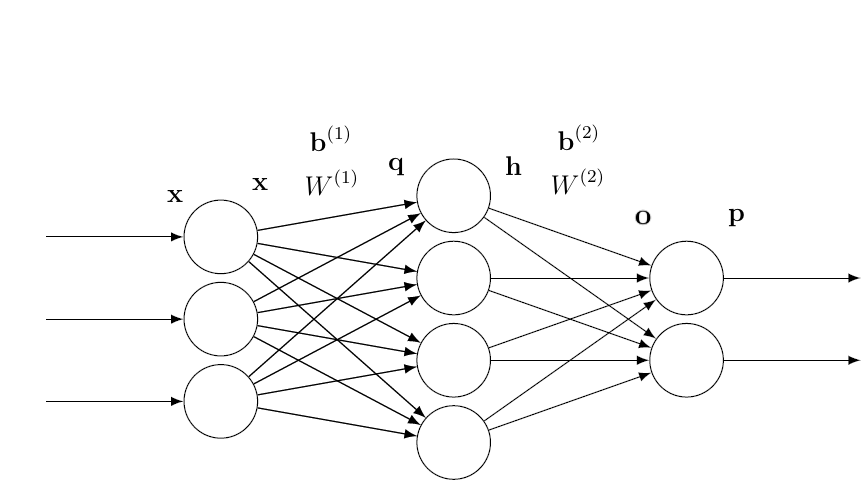
\includegraphics[width=0.9\textwidth]{images/neural-net.png}
    \caption{One layer fully connected neural network}
    \label{fig:my_label}
\end{figure}

\begin{align}
    \bq &= W^{(1)} \bx + \bb^{(1)} \\
    \bh &= \text{ReLU}(\bq)=\max{(0,\bq)} & \text{which is applied element-wise} \\
    \bo &= W^{(2)} \bh + \bb^{(2)} \\
    \bp &= \text{softmax}(\bo) & \text{which is defined as~}
    p_i = \frac{e^{o_i}}{\sum_{k=1}^M e^{o_k}} \\
    L(\bp, \by) &= - \sum_{i=1}^M y_i \log(p_i)
\end{align}

Note that $W^{(1)} \in \R^{H \times D}$, $\bb^{(1)} \in \R^H$, $W^{(2)} \in \R^{M \times H}$ and $\bb^{(2)} \in \R^M$.\par

Our ultimate goal is to calculate the gradients of the loss function with respect to the parameters $W^{(1)},\bb^{(1)},W^{(2)},\bb^{(2)}$. 

\clearpage


\subsection{(3 pts)}

In these sections, you may find it helpful to use the Kronecker delta (\url{https://en.wikipedia.org/wiki/Kronecker_delta}) as a shorthand. First, derive each of the following using chain rule:
\begin{align}
    \frac{\partial p_i}{\partial o_j},\ 
    \frac{\partial L}{\partial o_j},\ 
    \frac{\partial o_i}{\partial b_j^{(2)}},\ 
    \frac{\partial L}{\partial b_j^{(2)}}
\end{align}

\begin{soln}{height=10cm}
\ThreeAA
\end{soln}

Then, show that (by showing each element of the vectors are equal on both sides)
\begin{align}
    \nabla_\bo[L]=\bp - \by\\
    \nabla_{\bb^{(2)}}[L]=\bp - \by
\end{align}

\begin{soln}{height=5cm}
\ThreeAB
\end{soln}

\clearpage

\subsection{(3 pts)}

Derive the following using chain rule
\begin{align}
    \frac{\partial o_i}{\partial h_j},\ 
    \frac{\partial L}{\partial h_j}
\end{align}

\begin{soln}{height=11cm}
\ThreeBA
\end{soln}

Then, show that (by showing each element of the vectors are equal on both sides)
\begin{align}
    \nabla_{\bh} [L] &= W^{(2),\top}\nabla_{\bo}[L]
\end{align}
Note $W^{(2),\top}$ is the transpose of $W^{(2)}$\par

\begin{soln}{height=6cm}
\ThreeBB
\end{soln}

\clearpage

\subsection{(3 pts)}

Derive the following using chain rule
\begin{align}
    \frac{\partial o_k}{\partial W^{(2)}_{ij}},\ 
    \frac{\partial L}{\partial W^{(2)}_{ij}}
\end{align}

\begin{soln}{height=10cm}
\ThreeCA
\end{soln}

Then, show that (by showing each element of the matrices are equal on both sides) 
\begin{align}
    \nabla_{W^{(2)}} [L] = \nabla_\bo[L]\bh^{\top}
\end{align}

\begin{soln}{height=6cm}
\ThreeCB
\end{soln}

\clearpage

\subsection{(3 pts)}

Derive the following using chain rule. The second one should be in terms of $\frac{\partial L}{\partial h_i}$
\begin{align}
    \frac{\partial h_i}{\partial q_j},\ 
    \frac{\partial L}{\partial q_j}
\end{align}

\begin{soln}{height=12cm}
\ThreeD
\end{soln}

With these expressions at hand, you should be equipped to implement Problem $6$ efficiently. The derivative of $\bq$ with respect to $\bx$, $W^{(1)}$ and $\bb^{(1)}$ follows in the same way as $\bo$ with respect to $\bh$, $W^{(2)}$ and $\bb^{(2)}$.
\clearpage
\section{Convolution and Pooling (10 Points)}

\begin{figure}[H]
    \centering
    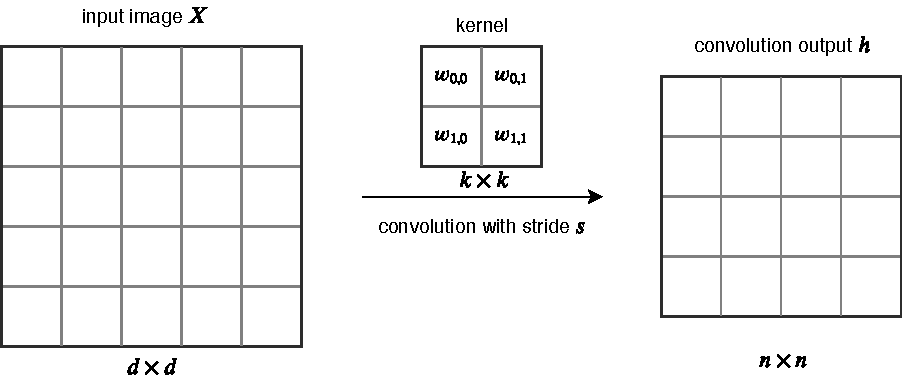
\includegraphics[width=0.7\textwidth]{images/conv.pdf}
    \caption{A simple example of convolution.}
    \label{fig:conv}
\end{figure}

In this problem, you will work on derivations of convolution. You will also get familiar with \texttt{im2col} (image to column), a popular technique to accelerate convolution. For this problem, assume padding = 0.

% \texttt{Im2col} is a method of representing convolution as matrix multiplication. Since we can do this, we know that convolution is a \textbf{linear operation}.\\

\subsection{(3 pts)} 
In lecture, you learned about two types of pooling as forms of downsampling: Max Pooling and Average Pooling
\begin{enumerate}
    \item
    Please show that \textbf{Average Pooling} is a linear operator by describing how it can be represented as a Convolution. In particular, for a square pooling field of shape $(p,p)$, please define the kernel matrix $A$ and stride $s$ needed to \textbf{implement Average Pooling as Convolution} for a one-channel input.
    \item
    Additionally, please explain why \textbf{Max Pooling} cannot be implemented as a convolution.
    \item
    Please say which you think would perform better and why: a CNN made up of \textbf{Convolutions and Max Pools} or a CNN made up of \textbf{Convolutions and Average Pools}.
\end{enumerate}
\newpage
    
\begin{soln}{height=10cm}
\FourA
\end{soln}
    

\subsection{(4 pts)} 

Let the input $X \in \mathbb{R}^{d\times d} $ be one single image, and is convolved by a $k\times k$ kernel with stride $s$. A simple example is shown in Figure \ref{fig:conv}.


\begin{enumerate}[label=\alph*.]
\item \textbf{(1 pts)} The convolution output is in the shape of $n\times n$. Can you represent the output dimensionality $n$ in terms of $d$, $k$ and $s$?

\begin{soln}{height=3cm}
\FourBA
\end{soln}
    
\item \textbf{(1 pts)} Denote the loss as $L$, convolution output as $h$, and kernel parameters as $w$. During backpropagation, given $\frac{\partial L}{\partial h_{i, j}}$ and input $X$, please derive $\frac{\partial L}{\partial w_{a, b}}$.

\begin{soln}{height=3cm}
\FourBB
\end{soln}

\pagebreak 
\item \textbf{(2 pts)} Can the above derivative be represented as a convolution? If so, write down its expression and define the corresponding kernel.

\begin{soln}{height=15cm}
\FourBC
\end{soln}

\end{enumerate}


\pagebreak

\subsection{(3 pts)}
In this part, you will be walked through \texttt{im2col} (image to column), and you are encouraged to use this technique in the programming exercise. Naively, an simple implementation of convolution would be sliding the kernel over the feature map. However, this would result in loops of all kernels and all locations, which is slow and can be accelerated by constructing two big matrices and going through one single matrix multiplication.

\begin{figure}[H]
    \centering
    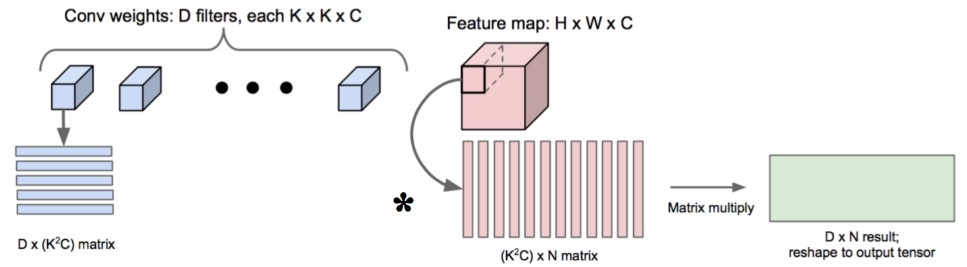
\includegraphics[width=0.9\textwidth]{images/im2col.jpg}
    \caption{Illustration of im2col.}
    \label{fig:im2col}
\end{figure}

An illustration of im2col is shown in Figure \ref{fig:im2col}. A patch inside the feature map corresponds to a possible location of the kernel. Each patch is of the same size as the convolution kernel, $K^2 C$, and $N$ is the number of all possible locations, or in other words, the spatial size of the output. We can take all possible patches, and reshape them into column vectors, then concatenate the vectors into one big matrix. Similarly, we can reshape the kernels into row vectors, and concatenate them into another one. Then we only need to go through one single matrix multiplication. And reshape the result to output shape.

For example, if the input feature map is of shape $32\times 32\times 3$, and we apply 5 filters each of size $5\times 5\times 3$ with stride=1 and padding=2, then the filter matrix would be of size $5\times 75$, and image matrix would be of size $75\times 1024$. The multiplication result would be of size $5\times1024$, and we need to reshape the result to shape $32\times 32\times 5$. (Hint: be very careful during reshaping.) 

\pagebreak

\begin{enumerate}[label=\alph*.]
\item \textbf{(2 pts)} Consider a toy example where the input feature map is of size $3\times3$, and convolved by 2 kernels of size $2\times2$ with stride $s=1$, as shown in Figure \ref{fig:toy_im2col}, please write the two constructed matrices with im2col.

\begin{figure}[H]
    \centering
    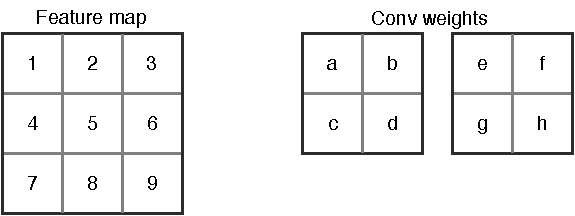
\includegraphics[width=0.5\textwidth]{images/im2col_toy_sample.pdf}
    \caption{A toy example of im2col}
    \label{fig:toy_im2col}
\end{figure}

% \item Problem about gradient.

\begin{soln}{height=5cm}
\FourCA
\end{soln}

\item \textbf{(1 pts)} Give one significant drawback of im2col.

\begin{soln}{height=5cm}
\FourCB
\end{soln}

\end{enumerate}
\clearpage
\section{MultiLayer Perceptron (30 pts)}

In this problem we will implement multi-layer perceptron for an image classification task. The data we use here is a subset of the CIFAR-10 dataset\footnote{\url{https://www.cs.toronto.edu/~kriz/cifar.html}}, where there are 10 classes of $32\times32$ images.

\fbox{%
    \parbox{\textwidth}{%
        \textbf{Warning: }It takes \textit{multiple hours} to train all of the  networks. Please start early and leave ample time for training/debugging. Be sure to \textit{vectorize} all of your computations to ensure they can run fast enough (so make computations in the form of vector and matrix multiplications as much as possible instead of for loops).\\\\
        In \textbf{Problem 5 and 6}, you will first implement several classes of important neural network modules, and then use these modules to build up the networks. For this part, we provide a template code. Please FOLLOW the templates, and implement the classes methods. Do NOT change the interface. The classes will be used for auto-grading. Code that does not pass the autograder WILL NOT be graded.
    }%
}

{\bf Format of the data}: 
The dataset are stored in a pickle file (\texttt{cifar10-subset.pkl}), which can be downloaded from the ``Resources'' tab on piazza. There are 5000 images for training and 2000 images for testing, each corresponding to an ``integer'' label (in range $0$ to $9$). Once you download the dataset, replace \texttt{CIFAR\_FILENAME} in the main function by the relative path you store the pickle file. \texttt{trainX} is a numpy array of dimension $(5000, 3072)$ representing the 5000 training images, and \texttt{trainy} is a $(5000, 10)$ dimensional numpy array of one-hot vectors representing the corresponding label information. Similarly, \texttt{testX} and \texttt{testy} contain $2000$ data points and use the same format as the training dataset (i.e, $(2000, 3072)$ dimensional array and $(2000, 10)$ dimensional array). Normalizing the input (\texttt{trainX}, \texttt{testX}) to [0, 1] and converting the input to numpy array of float32 can accelerate training.

The label mappings are:
\begin{verbatim}
    { 
      0: `Airplane', 
      1: `Automobile',
      2: `Bird',
      3: `Cat',
      4: `Deer',
      5: `Dog',
      6: `Frog',
      7: `Horse',
      8: `Ship',
      9: `Truck',
    }
\end{verbatim}

%The data is stored in multiple pickle files, with 10000 images for training and 2500 for testing. It can be found on Piazza under the Resources tab. Once you download the dataset, replace \texttt{SVHN\_DOWNLOAD\_PATH} of \texttt{load\_svhn.py} with the directory where you extracted the dataset. Each image's class corresponds to a specific digit (ranging from $0$ to $9$). \texttt{train\_X.npy} is a Numpy array of dimension $(10000, 3072)$ representing the 10000 training images, and \texttt{train\_y.npy} is a $(10000,)$ dimensional Numpy vector containing the corresponding labels for the images. Similarly, \texttt{test\_X.npy} and \texttt{test\_y.npy} contain $2500$  datapoints and use the same format as the training dataset (i.e, $(2500 \times 3072)$ dimensional array and $(2500,)$ dimensional vector). The pixel values of the images (\texttt{train\_X}, \texttt{test\_X}) are already normalized to [0, 1].


% \footnote{Download: \url{https://drive.google.com/drive/folders/1y1s2ddGSgClJbd3QHHqHS12lNe48q7vx?usp=share_link}}

As a warm up practice (not graded), we recommend loading the data and plotting a few examples. 

\textbf{For problems 5 and 6, submit \texttt{mlp.py} and \texttt{cnn.py} only to gradescope (select them simultaneously and drag them to upload).}



\subsection{Implementation (15 pts)}

In the Problem 5 folder, \textbf{mlp.py} is the only file you need to work on. \textbf{tests.py} and \textbf{tests.pk} are to help you test your implementation locally. Passing these local tests does not guarantee you passing the final online auto-grading tests, but failing locally very likely means also failing online. The following are terminal commands to run single module test and all modules test. 
\begin{verbatim}
    python -m unittest tests.TestReLU
    python -m unittest tests
\end{verbatim}

In \textbf{mlp.py}, there is a base class called \texttt{Transform} which you do not need to change. The \texttt{Transform} class represents a procedure done to some input $X$. In symbolic terms, $out = f(X)$, where $f$ represents the transformation, $y$ the output, $x$ the input. We will be implementing the basic layers (e.g. \texttt{ReLU}, \texttt{LinearMap}, etc.) of neural networks by inheriting this \texttt{Transform} base class.


Below is a list of classes we will implement. Implement wherever the code template says \texttt{pass}. Reading \texttt{tests.py} might help you debug your implementation. 

\begin{itemize}
    \item {\bf ReLU} ({\bf 1 point}): The layer of Rectified Linear Unit, a popular activation function. Available unit tests: \texttt{TestReLU};
    
    \item {\bf LinearMap} ({\bf 3 points}): Linear Transformation layer, i.e. fully-connected layer. In parameter update function \texttt{step()}, parameters should be updated using gradient descent with momentum. Available unit tests: \texttt{TestLinearMap};
    
    \item {\bf SoftmaxCrossEntropyLoss} ({\bf 2 points}): The layer of softmax and cross-entropy loss. The input is the pre-softmax logits, and the output is the \textbf{mean} cross-entropy loss across samples in a batch. Available unit tests: \texttt{TestLoss};
    
    \item {\bf SingleLayerMLP} ({\bf 3 points}): This is a nerual network with one hidden layer. The output is the logits(pre-softmax) for the classification tasks. Available unit tests: \texttt{TestSingleLayerMLP};
    
    \item {\bf TwoLayerMLP} ({\bf 3 points}): This is a neural network with two hidden layers. The output is the logits(pre-softmax) for the classification tasks. Available unit tests: \texttt{TestTwoLayerMLP}.
    
    \item {\bf Dropout} ({\bf 1 point}): The dropout layer. In this assignment, we apply mask and scaling during training and do nothing at test time. Available unit tests: \texttt{TestDropout}.
    
    \item {\bf BatchNorm} ({\bf 2 points}): The batch normalization layer. Please refer to the batch normalization paper or this\footnote{\url{https://agustinus.kristia.de/techblog/2016/07/04/batchnorm/}} for implementation. Available unit tests: \texttt{TestBatchNorm}.
\end{itemize}
\pagebreak
\textbf{Tips}:
\begin{itemize}
    \item LinearMap layer weights should be initialized using Xavier Initialization:
        \[W^k_{i,j}\sim\texttt{Uniform}(-b,b) \;,\quad b=\sqrt{\frac{6}{m+n}}\]
     where $k$, $i$, $j$ are indices for network layer and nodes, $m$ and $n$ are the input and output dimension;
    \item Special practices might be necessary for the numerical stability of the Softmax function;
   % \item You can start with these hyperparamters. Learning rate: 0.001, $\alpha$: 0.9 (parameter for momentum), batch size: 128. Other hyperparameters very likely could give better performance. Hyperparameters should be consistent when you compare different network architectures. 
\end{itemize}

This is what the TwoLayer network would look like:\\
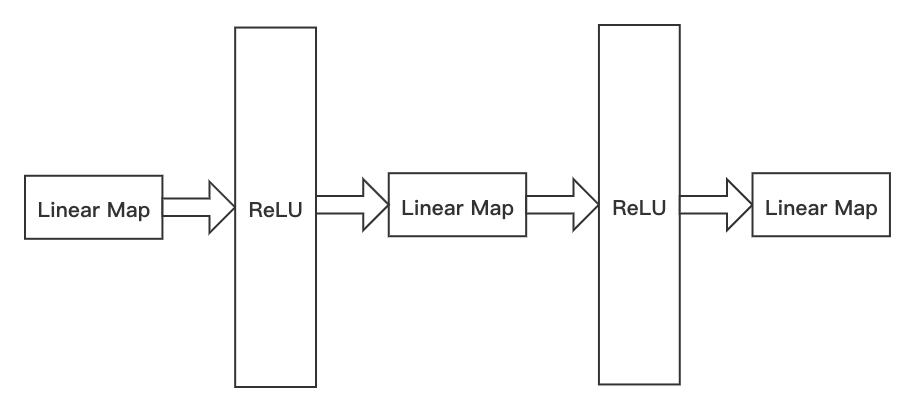
\includegraphics[scale=0.5]{images/onetask.png}


\subsection{Experiments (15 pts)}
In this section, we will train and test the two networks we implemented, and evaluate their performances.  

The network models will take images as inputs and give softmax output over 10 classes. During training, we will perform gradient descent with momentum to minimize Cross-Entropy Loss. Run the optimization for \textcolor{blue}{50} epochs each time. Using the following hyperparameters parameters for training: batch size = $128$, learning rate = $0.001$, momentum = $0.9$. %If you observe underfitting, continue training for more epochs until overfitting.

For every architecture, plot the train and test loss together on one plot, with loss on the y-axis against epoch number on x-axis. Similarly, plot the train and test accuracy after every epoch. Label each curve and all axes. Report the best loss and accuracy for training and testing achieved.

\pagebreak

\begin{enumerate}
    \item \textbf{(5 pts)} Train a \textbf{SingleLayerMLP} with $800$ hidden nodes, show plots of loss and accuracy, and report the best loss and accuracy achieved.
    \begin{soln}{height=9cm}
    \FiveBA
    \end{soln}

    \item \textbf{(5 pts)} Train a \textbf{TwoLayerMLP} with $(800, 800)$ hidden nodes, show plots of loss and accuracy, and report the best loss and accuracy achieved.
    \begin{soln}{height=9cm}
    \FiveBB
    \end{soln}
    \newpage
    
    \item \textbf{(3 pts)} Batch Normalization: To the \textbf{SingleLayerMLP} in Problem 1, implement batch normalization using the same batch size as in Problem 1. Describe how batch norm helps (or doesn't help) in terms of speed and accuracy (train and validation).
    \begin{soln}{height=9cm}
    \FiveBC
    \end{soln}

    \item \textbf{(2 pts)}  Dropout: Now, to the \textbf{SingleLayerMLP} of Problem 1, add a dropout to the output of layer 1 with a probability of 0.5 and report your findings. Do you observe any changes in terms of performance? Does a model trained with dropout perform better or worse than the SingleLayerMLP? Briefly explain why you think this happens.
    \begin{soln}{height=9cm}
    \FiveBD
    \end{soln}

\end{enumerate}
\clearpage
\section{Convolutional Neural Network (35 pts)}

In this problem we will implement convolutional neural networks for an image classification task. The data is the same as in the previous problem. 

Again, the dataset is stored in a pickle file, with 5000 images for training and 2000 for testing. Once you download the dataset, replace \texttt{CIFAR\_FILENAME} in the main function with the path where you stored the dataset and it would load the data for you. This time, the data is prepared in the following format:

\texttt{trainX} / \texttt{testX} -- $(5000/2000, 3, 32, 32)$ numpy array of images normalized to [0, 1].\newline
\texttt{trainy} / \texttt{testy} -- $(5000/2000, 10)$ numpy array of one-hot vectors representing labels.

\subsection{Implementation (16 pts)}

In the Problem 6 folder, \textbf{cnn.py} is the only file you need to work on. \textbf{tests.py} and \textbf{tests.pk} are to help you test your implementation locally. Passing these local tests does not guarantee you passing the final online auto-grading tests, but failing locally very likely means also failing online. The following are terminal commands to run single module test and all modules test. 
\begin{verbatim}
    python -m unittest tests.TestReLU
    python -m unittest tests
\end{verbatim}

% \subsubsection*{1.2 Backpropagation Algorithm for CNNs}
Below is a list of classes we will implement. Implement wherever the code template says \texttt{pass}. Reading \texttt{tests.py} might help you debug your implementation. 

\begin{itemize}

    \item {\bf ReLU} ({\bf 0 points}): ReLU layer. Available unit tests: \texttt{TestReLU}.
    
    \item {\bf Conv} ({\bf 7 points}): Convolutional layer. You will also need to implement functions \textbf{im2col} and \textbf{im2col\_bw} in order to vectorize the forward and backward computation of convolutional layer 
    \footnote{The following links from the cs231n course at Stanford are very helpful: \url{http://cs231n.stanford.edu/slides/2016/winter1516_lecture11.pdf}(starting on slide 66) and \url{http://cs231n.github.io/convolutional-networks/}}.  
    Available unit tests: \texttt{TestIm2Col}, \\ \texttt{TestConvWeightsBias}, \texttt{TestConvForward}, \texttt{TestConvBackward} and \texttt{TestConvUpdate}.
    
    \item {\bf Maxpool} ({\bf 4 points}): Max Pooling layer. Available unit tests: \texttt{TestMaxPoolForward} and \texttt{TestMaxPoolBackward}.
    
    \item {\bf LinearLayer} ({\bf 2 points}): Fully Connected layer, or Linear Layer. Available unit tests: \texttt{TestFCWeightsBias}, \texttt{TestLinearForward}, \texttt{TestLinearBackward} and \texttt{TestLinearUpdate}.
    
    \item {\bf SoftMaxCrossEntropyLoss} ({\bf 0 points}): The layer of softmax and cross-entropy loss. The input is the pre-softmax logits, and the output is the \textbf{mean} of cross-entropy loss across samples in a batch. 

    \item {\bf ConvNet} ({\bf 3 points}): This is where you will initialize and call all the previous layers to implement the convolutional network. Available unit tests: \texttt{TestConvNet}.
    
\end{itemize}
\pagebreak
\textbf{Tips}:
\begin{itemize}
    \item Linear layer weights initialization is the same with Problem 5. Convolutional layer weights should be initialized as: \[W^k_{i,j}\sim\texttt{Uniform}(-b,b) \;,\quad b=\sqrt{\frac{6}{(f+c)*h*w}}, \]
    where $k$, $i$, $j$ are indices for network layer and nodes, $f$ the number of filters (the number of output channels), $c$ the number of input channels, $h$ and $w$ the filter height and width.
    %\item You can start with these hyperparamters. Learning rate: 0.001, Momentum: 0.9, Batch size: 128. Other hyperparameters very likely could give better performance. Hyperparameters should be consistent when you compare different network architectures. 
\end{itemize}

\subsection{Experiments (19 pts)}
In this section, you will implement different network architectures to see how they affect the performance. 

The network models will take images as inputs and give softmax output over 10 classes. During training, we will perform gradient descent with momentum to minimize Cross-Entropy Loss. Run the optimization for \textcolor{blue}{50} epochs each time. Using the following hyperparameters parameters for training: batch size = $128$, learning rate = $0.001$, momentum = $0.9$. %If you observe underfitting, continue training for more epochs until overfitting. 

\begin{enumerate}
    \item \textbf{(12 pts)} For every architecture, plot the train and test loss together on one plot, with loss on the y-axis against epoch number on x-axis. Similarly, plot the train and test accuracy after every epoch. Label each curve and all axes. Report the best loss and accuracy for training and testing achieved.
    
    For those with CNN layers, the stride is 1 and the padding size is 2.
    
    \pagebreak

    \begin{enumerate}
        \item \textbf{1conv1filter (3 pts)} 
            A convolutional layer with one $6\times6$ filter and ReLU activation, a $2\times2$ max pooling layer, a linear layer, a softmax layer.

            \textit{Hint: This simple architecture is mostly for helping you debug your convolutional layer. There is no need to worry about poor performance as long as  it significantly improves for the next two architectures.}
            
            \begin{soln}{height=9cm}
            \SixBAA
            \end{soln}
            
        \item \textbf{1conv5filter (3 pts)}
            A convolutional layer with five $4\times4$ filters and ReLU activation, a $2\times2$ max pooling layer, a linear layer, a softmax layer.
            
            \begin{soln}{height=9cm}
            \SixBAB   
            \end{soln}
    
        \item \textbf{3conv5filter (3 pts)}
            A convolutional layer with five $4\times4$ filter and ReLU activation, a $2\times2$ max pooling layer, a convolutional layer with five $4\times4$ filter and ReLU activation, a convolutional layer with five $4\times4$ filter and ReLU activation, a linear layer, a softmax layer.
            
            \begin{soln}{height=8cm}
            \SixBAC
            \end{soln}
            
        \item \textbf{Full comparison between MLP and CNN (3 pts)}
            Plot the test accuracy for all the experiments you have done so far for both MLP and CNN. Also, explain why you think one has better performance than the other.\\\textit{Hint: Look at the number of parameters of each network}.
            
            \begin{soln}{height=9cm}
            \SixBAD
            \end{soln}
            
    \end{enumerate}
    
    \pagebreak
    
    \item \textbf{(7 pts)} Compare different architectures based on your own results. 
    \begin{enumerate}
            \item Compare (a) and (b). (2 pts)
                \begin{soln}{height=4cm}
                \SixBBA
                \end{soln}

            \item Compare (b) and (c). (2 pts)
                \begin{soln}{height=4cm}
                \SixBBB
                \end{soln}

            \item Compare the best CNN model with the best MLP model. (2 pts)
                \begin{soln}{height=4cm}
                \SixBBC
                \end{soln}

            \item Which one is your best performing CNN network (on the test dataset)? (1 pt)
                \begin{soln}{height=4cm}
                \SixBBD
                \end{soln}
    \end{enumerate}
    

\end{enumerate}



\clearpage
\textbf{Collaboration Questions} Please answer the following:


After you have completed all other components of this assignment, report your answers to the collaboration policy questions detailed in the Academic Integrity Policies found \href{http://www.cs.cmu.edu/~mgormley/courses/10601bd-f18/about.html#7-academic-integrity-policies}{here}.
\begin{enumerate}
    \item Did you receive any help whatsoever from anyone in solving this assignment? Is so, include full details.
    \item Did you give any help whatsoever to anyone in solving this assignment? Is so, include full details.
    \item Did you find or come across code that implements any part of this assignment ? If so, include full details even if you have not used that portion of the code. 
\end{enumerate}

\begin{soln}{height=10cm}
\Collaboration
\end{soln}
\clearpage


\end{document}